\scanpage{123}
% archive foliation: 122
\diagram{\begin{tikzcd}[ampersand replacement=\&,column sep=small]
\zeta_1\arrow[d,mapsto]\&\zeta_2\arrow[d,mapsto]\&\zeta_3\arrow[d,mapsto]\&{}\in k\&\&\infty\arrow[dll,bend right=20,mapsto]\\
0\&1\&\infty\&t\&\&
\end{tikzcd}}

\[
\left\{\begin{array}{l}\zeta_1,1\\\zeta_2,1\\\zeta_3,1\end{array}\right.
\]

\figure{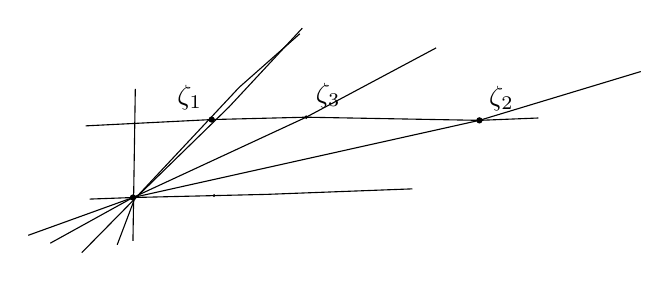
\begin{tikzpicture}[x=1cm,y=1cm]
\draw (-.65,-.7)--(.02,-.02)--(1.35,1.4)--(2.12,2.08);
\draw (-.2,-.6)--(.02,-.02)--(1.22,1.15)--(2.15,2.15);
\draw (-1.05,-.58)--(0,0)--(2.2,1.02)--(3.85,1.9);
\draw (-1.33,-.48)--(0,0)--(4.4,.98)--(6.45,1.6);
\draw (-.55,-.02)--(0,0)--(1.7,.04)--(3.55,.11);
\draw (0,-.55)--(.03,1.38);
\draw (-.6,.91)--(1,.99)--(2.2,1.02)--(4.4,.98)--(5.15,1.01);
\fill (0,0) circle(.04);
\fill (1,.99) circle(.04) node[above left] {$\zeta_1$};
\fill (2.2,1.02) circle(.025) node[above right] {$\zeta_3$};
\fill (4.4,.98) circle(.04) node[above right] {$\zeta_2$};
\fill (1.03,.025) circle(.02);
\end{tikzpicture}}

\[
\begin{array}{l}
\lambda_1\zeta_1,\lambda_1\\
\lambda_2\zeta_2,\lambda_2\\
\lambda_3\zeta_3,\lambda_3
\end{array}
\qquad
\left[\begin{gathered}
\sum\lambda_i=0\\
\sum\lambda_i\zeta_i=0\\
\text{Cela détermine }(\lambda_i)\text{ mod }\inserted{\text{mult. par}}\text{ scalaire inv.}
\end{gathered}\right.
\]
$\zeta_1,\zeta_2,\zeta_3$ tous distincts

\unsure{Or}
\[
\begin{array}{l|l}
\lambda_1=\zeta_{\underline2}-\zeta_{\underline3}&\zeta_1\\
\lambda_2=\zeta_{\underline3}-\zeta_{\underline1}&\zeta_2\\
\lambda_3=\zeta_{\underline1}-\zeta_{\underline2}&\zeta_3
\end{array}
\qquad
\left\{\begin{aligned}
\deleted{\unsure{e_2}}-e_3&=((\zeta_2-\zeta_3)\zeta_1,\zeta_2-\zeta_3)\\
\deleted{\unsure{e_3}}-e_1&=((\zeta_3-\zeta_1)\zeta_2,\zeta_3-\zeta_1)\\
\deleted{\unsure{e_1}}-e_2&=((\zeta_1-\zeta_2)\zeta_3,\zeta_1-\zeta_2)
\end{aligned}\right.
\]
\deleted{$\unsure{e_3}$}
\diagram{\begin{tikzcd}[ampersand replacement=\&]
f_1\arrow[r]\&{}
\end{tikzcd}}
\diagram{\begin{tikzcd}[ampersand replacement=\&]
(\zeta_1,1)\arrow[r,|-]\&\zeta_1f_1+
\end{tikzcd}}
